% Lec. 5: Normal Modes — Friday, January 10, 2025

\chapter{Normal Modes, Gravity, and the Virial Theorem}

\section{Normal Coordinates}

\[
    x_i = \sum_j C_{ij} q_j \qquad \text{(linear combination of coordinates)}
\]

For linear systems,
\[
    \Rightarrow\quad \alpha_i \ddot{x}_i + \beta_i \dot{x}_i + \gamma x_i = f_i(t)
\]

\subsection{Example: Mechanical Vibrations in Molecules}

\begin{figure}[H]
\begin{center}
\begin{tikzpicture}
\begin{axis}[
  width=0.5\textwidth, height=4.5cm,
  xlabel={$r$}, ylabel={$U(r)$},
  xmin=0.5, xmax=5, ymin=-1.5, ymax=2.0,
  xtick={1.5}, xticklabels={$r_0$},
  ytick={0,-1.0}, yticklabels={$0$,$U_\text{min}$},
  axis lines=left, samples=150,
]
  % Lennard-Jones like potential
  \addplot[thick,blue,domain=0.72:5]{(1/(x^6)) - (1.5/x^2) + 0.1};
  % Minimum marker
  \addplot[only marks,mark=*,mark size=2pt,red] coordinates {(1.5,-0.98)};
  \draw[dashed,gray] (axis cs:1.5,2.0) -- (axis cs:1.5,-0.98);
  % Harmonic approximation (parabola near minimum)
  \addplot[thick,dashed,red,domain=0.9:2.1]{-0.98 + 3.0*(x-1.5)^2}
    node[pos=0.85,right,scale=0.8]{$\approx \tfrac{1}{2}k(r-r_0)^2$};
  % Zero level
  \addplot[dashed,gray,domain=0.5:5]{0};
\end{axis}
\end{tikzpicture}
\end{center}
\caption{Interatomic potential $U(r)$ vs.\ separation $r$, showing a minimum at equilibrium distance $r_0$. Near the minimum, $U$ is well approximated by a parabola (harmonic approximation, red dashed).}
\label{fig:interatomic_pot}
\end{figure}

\begin{itemize}
    \item Potential is about $r_0$ constant (i.e.\ $\approx 0$ to first order).
    \item Taylor expand about equilibrium $r_0$:
    \[
        U(r - r_0) \approx U(r_0) + \left.\frac{\partial U}{\partial r}\right|_{r=r_0}(r - r_0)
        + \frac{1}{2}\left.\frac{\partial^2 U}{\partial r^2}\right|_{r=r_0}(r-r_0)^2 + \cdots
    \]
    The first-order term vanishes at equilibrium; the second-order coefficient is $> 0$ because it is a stable equilibrium.
\end{itemize}

Thus for \underline{any} system that is near a stable equilibrium point,

\begin{formula}[Harmonic approximation near equilibrium]
\[
    U(r) \approx \tfrac{1}{2}k(r - r_0)^2
\]
\end{formula}

\subsection{Example: CO\textsubscript{2} molecule ($\text{C} = \text{O} = \text{C}$)}

\begin{figure}[H]
\begin{center}
\begin{tikzpicture}[scale=1.0, >=Stealth]
  % Wall anchors (none needed — free molecule)
  % Atom O (left)
  \fill[red!70] (0,0) circle[radius=0.25];
  \node[below] at (0,-0.3) {O};
  \node[above,scale=0.8] at (0,0.3) {$m_O$};
  % Displacement x1 arrow
  \draw[->,blue,thin] (0,-0.55) -- (0.4,-0.55) node[right,scale=0.8]{$x_1$};
  % Spring 1
  \draw[thick, decorate, decoration={zigzag,segment length=5pt,amplitude=3pt}]
    (0.25,0) -- (1.75,0);
  \node[above,scale=0.8] at (1.0,0.2) {$k$};
  % Atom C (centre)
  \fill[gray!70] (2.0,0) circle[radius=0.2];
  \node[below] at (2.0,-0.3) {C};
  \node[above,scale=0.8] at (2.0,0.3) {$m_C$};
  % Displacement x2 arrow
  \draw[->,blue,thin] (2.0,-0.55) -- (2.4,-0.55) node[right,scale=0.8]{$x_2$};
  % Spring 2
  \draw[thick, decorate, decoration={zigzag,segment length=5pt,amplitude=3pt}]
    (2.2,0) -- (3.75,0);
  \node[above,scale=0.8] at (3.0,0.2) {$k$};
  % Atom O (right)
  \fill[red!70] (4.0,0) circle[radius=0.25];
  \node[below] at (4.0,-0.3) {O};
  \node[above,scale=0.8] at (4.0,0.3) {$m_O$};
  % Displacement x3 arrow
  \draw[->,blue,thin] (4.0,-0.55) -- (4.4,-0.55) node[right,scale=0.8]{$x_3$};
\end{tikzpicture}
\end{center}
\caption{CO$_2$ modelled as three masses connected by two springs of spring constant $k$: O--spring--C--spring--O. Displacements $x_1$, $x_2$, $x_3$ are measured from equilibrium positions.}
\label{fig:co2_springs}
\end{figure}

\begin{itemize}
    \item Treat atoms as point particles.
    \item Total DOF: $3 \times 3 = 9$ normal modes \quad (3 atoms $\times$ 3 spatial coords).
    \item But there will be 3 trivial translation modes $\Rightarrow 9 - 3 = 6$.
    \item Also there are 2 rotation modes $\Rightarrow 6 - 2 = 4$ normal modes for vibrations.
\end{itemize}

The Lagrangian (considering only 1D motion along the axis, with oxygen masses $m_O$ and carbon mass $m_C$):
\[
    L = \tfrac{1}{2}m_O(\dot{x}_1^2 + \dot{x}_3^2) + \tfrac{1}{2}m_C(m_C \dot{x}_2^2)
        - \tfrac{1}{2}k(x_2 - x_1)^2 - \tfrac{1}{2}k(x_3 - x_2)^2
\]

Applying the Euler--Lagrange equation for $x_1$:
\[
    \frac{\partial L}{\partial x_1} - \frac{d}{dt}\frac{\partial L}{\partial \dot{x}_1} = 0
    = -k(x_1 - x_2) - \frac{d}{dt}(m_O \dot{x}_1)
    \quad\Rightarrow\quad
    \ddot{x}_1 + \frac{k}{m_O}(x_1 - x_2) = 0 \tag{1}
\]

By $x_1 \leftrightarrow x_3$ symmetry:
\[
    \ddot{x}_3 + \frac{k}{m_O}(x_3 - x_2) = 0 \tag{3}
\]

For $x_2$:
\[
    \frac{\partial L}{\partial x_2} - \frac{d}{dt}\frac{\partial L}{\partial \dot{x}_2} = 0
    \quad\Rightarrow\quad
    \ddot{x}_2 + \frac{k}{m_C}(2x_2 - x_2 - x_3) \tag{2}
\]

\textbf{Ansatz:} Try $x_i = C_i e^{i\omega t}$.

Plugging into (1):
\[
    -\omega^2 C_1 e^{i\omega t} + \frac{k}{m_O}(C_1 - C_2)e^{i\omega t} = 0
\]
\[
    (2): \quad -\omega^2 C_2 e^{i\omega t} + \frac{k}{m_C}(2C_2 - C_1 - C_3)e^{i\omega t} = 0
\]
\[
    (3): \quad -\omega^2 C_3 e^{i\omega t} + \frac{k}{m_O}(C_3 - C_2)e^{i\omega t} = 0
\]

Writing in matrix form:
\[
    \begin{pmatrix}
        \dfrac{k}{m_O} - \omega^2 & -\dfrac{k}{m_O} & 0 \\[8pt]
        -\dfrac{k}{m_C} & \dfrac{2k}{m_C} - \omega^2 & -\dfrac{k}{m_C} \\[8pt]
        0 & -\dfrac{k}{m_O} & \dfrac{k}{m_O} - \omega^2
    \end{pmatrix}
    \begin{pmatrix} C_1 \\ C_2 \\ C_3 \end{pmatrix}
    =
    \begin{pmatrix} 0 \\ 0 \\ 0 \end{pmatrix}
\]

Set $\det A = 0$:
\[
    \left(\frac{k}{m_O} - \omega^2\right)
    \left[\left(\frac{2k}{m_C} - \omega^2\right)\left(\frac{k}{m_O} - \omega^2\right)
    - \frac{k^2}{m_O m_C}\right]
    + \frac{k}{m_O}\cdot\frac{-k}{m_C}\left(\frac{k}{m_O} - \omega^2\right) = 0
\]
\[
    \omega^2\left(\frac{k}{m_O} - \omega^2\right)\left(\omega^2 - \frac{2k}{m_C} - \frac{k}{m_O}\right) = 0
\]

\textbf{Solutions:}

\begin{itemize}
    \item $\omega^2 = 0 \Rightarrow C_1 = C_2 = C_3$ $\Rightarrow$ linear translation.
    \[
        \begin{pmatrix}0\\0\\0\end{pmatrix} \quad \lambda = 7\,\mu\text{m}
    \]

    \item $\omega_a^2 = \dfrac{k}{m_O} \Rightarrow C_2 = 0,\; C_1 = -C_3 \Rightarrow x_1(t) = -x_3(t)$.
    \[
        \begin{pmatrix}1\\0\\-1\end{pmatrix} \quad \lambda_a = \text{DNE (no dipole, because no displacement of C)}
    \]

    \item $\omega_b^2 = \left(\dfrac{2k}{m_C} + \dfrac{k}{m_O}\right)
    \Rightarrow C_2 = -\dfrac{2m_O}{m_C}C_1,\; C_1 = C_3$.
    \[
        x_1(t) = x_3(t), \quad x_2(t) = -\frac{2m_O}{m_C}x_1(t)
        \quad\Rightarrow\quad
        \begin{pmatrix}1 \\ -\frac{2m_O}{m_C} \\ 1\end{pmatrix}e^{i\omega t}
        \quad \lambda_b = 4\,\mu\text{m}
    \]
\end{itemize}

\begin{example}[Application: QM absorption lines]
In QM, $\lambda = \dfrac{2\pi c}{\omega}$. We know $k \sim 140\,\text{eV}$.
Based on whether a dipole moment forms, we can calculate absorption lines of molecules.
\end{example}

\subsection{2D Molecule Modes}

Look for modes where the center of mass doesn't move.

\begin{figure}[H]
\centering
\caption{A bent triatomic molecule with two outer atoms (mass $m_O$) displaced transversely by $y$, and the central atom (mass $m_C$) displaced by $y_2$ vertically. The bonds make an angle with the horizontal.}
\end{figure}

COM condition:
\[
    m_O(-y - y) + m_C y_2 = 0 \quad\Rightarrow\quad y_2 = \frac{2m_O}{m_C}y
\]

The Lagrangian (with $k_\perp$ the transverse spring constant, noting there is only one oscillation so no double-counting):
\begin{align*}
    L &= 2 \cdot \tfrac{1}{2}m_O \dot{y}^2 + \tfrac{1}{2}m_C\left(\frac{2m_O}{m_C}\dot{y}\right)^2
    - \tfrac{1}{2}k_\perp\left[2\left(y + \frac{2m_O}{m_C}y\right)\right]^2 \\
    &= \dot{y}^2\left(m_O + \frac{2m_O^2}{m_C}\right) - 2k_\perp\left(1 + \frac{2m_O}{m_C}\right)^2 y^2
\end{align*}

Applying the Euler--Lagrange equation:
\[
    \frac{\partial L}{\partial y} - \frac{d}{dt}\frac{\partial L}{\partial \dot{y}}
    = -4k_\perp y\left(1 + \frac{2m_O}{m_C}\right)^2 - \frac{d}{dt}\left[2\dot{y}\,m_O\!\left(1 + \frac{2m_O}{m_C}\right)\right]
\]
\[
    \Rightarrow\quad \ddot{y} + 2k_\perp\left(\frac{1}{m_O} + \frac{2}{m_C}\right)y = 0
\]
\[
    \Rightarrow\quad \omega_\perp^2 = 2k_\perp\left(\frac{1}{m_O} + \frac{2}{m_C}\right)
\]

% -------------------------------------------------------
% Lec. 6: Gravity — Monday, January 13, 2025
% -------------------------------------------------------

\chapter{Gravity and Orbital Mechanics}

\section{Kepler's Laws (Empirical)}

\begin{enumerate}
    \item The orbit of every planet is an ellipse with the Sun at one of the two foci.
    \item A line joining a planet to the Sun sweeps out equal area in equal time.
    \item $T^2 \sim (\text{semi-major axis length})^3$.
\end{enumerate}

\begin{itemize}
    \item Any time you have a point source that radiates uniformly, the density goes like $r^{-2}$ (because surface area is $4\pi r^2$).
    \item Gravity can be thought of like radiation.
\end{itemize}

\section{Newton's Argument}

Near the surface of the Earth:
\[
    mg = \frac{G M_E m}{r^2} \quad \text{($G M_E$ unknown)}
\]

For the Moon in circular orbit:
\[
    m_m \frac{v_m^2}{D_{e\text{-}m}} = \frac{G M_E m_m}{D_{e\text{-}m}^2}, \qquad v_m = \frac{2\pi D_{e\text{-}m}}{T_m}
\]
\[
    \Rightarrow\quad \frac{4\pi^2 D_{e\text{-}m}}{T_m^2} = \frac{G M_E}{D_{e\text{-}m}} = \frac{g R_E^2}{D_{e\text{-}m}}
\]
\[
    \Rightarrow\quad
    \boxed{T_m \stackrel{?}{=} \frac{2\pi D_{e\text{-}m}^{3/2}}{R_E \sqrt{g}}}
\]
This is testable because $g$, $R_E$, $T_m$ are known; you can use parallax to measure distance to the Moon.

\begin{example}[Eratosthenes]
Precise measurement of the radius of the Earth.
\[
    R_E = \frac{D}{\theta}
\]
\begin{figure}[H]
\centering
\caption{Two observers separated by distance $D$ on the Earth's surface measure the Sun at different angles; the central angle $\theta$ gives $R_E = D/\theta$.}
\end{figure}
\end{example}

\section{Two-Body Orbital Problem}

\begin{figure}[H]
\centering
\caption{Two masses $m_1$ and $m_2$ in the COM frame, with separation $r$ and angle $\theta$. Distances from COM: $\frac{m_2}{M}r$ for $m_1$ and $\frac{m_1}{M}r$ for $m_2$.}
\end{figure}

\begin{itemize}
    \item Consider the COM frame: $\sum p_i = 0$ (conserved momentum).
    \item Distances from COM are as follows (with $M = m_1 + m_2$):
    \[
        r_1 = \frac{m_2}{M}r, \qquad r_2 = \frac{m_1}{M}r
    \]
    \item Motion must be confined to a plane (in this case the board) --- no out-of-plane motion.
\end{itemize}

\begin{align*}
    L &= \tfrac{1}{2}m_1\left[\left(\frac{m_2}{M}\dot{r}\right)^2 + \left(\frac{m_2}{M}r\dot\theta\right)^2\right]
       + \tfrac{1}{2}m_2\left[\left(\frac{m_1}{M}\dot{r}\right)^2 + \left(\frac{m_1}{M}r\dot\theta\right)^2\right]
       + \frac{Gm_1 m_2}{r} \\
    &= \frac{m_1 m_2}{2M^2}\left[\dot{r}^2(m_2 + m_1) + r^2\dot\theta^2(m_2 + m_1)\right] + \frac{Gm_1 m_2}{r}
\end{align*}

Define the \emph{reduced mass}:
\begin{formula}[Reduced mass]
\[
    \frac{1}{\mu} = \frac{1}{m_1} + \frac{1}{m_2} = \frac{M}{m_1 m_2}
    \quad\Rightarrow\quad \mu = \frac{m_1 m_2}{M}
\]
\end{formula}

\[
    \Rightarrow\quad L = \tfrac{1}{2}\mu(\dot{r}^2 + r^2\dot\theta^2) + \frac{Gm_1 m_2}{r}
\]

This is equivalent to a single particle of mass $\mu$ at distance $r$ from the origin in a gravitational field.

\subsection{Conservation of Angular Momentum}

\[
    \frac{\partial L}{\partial \theta} - \frac{d}{dt}\frac{\partial L}{\partial \dot\theta}
    = 0 - \frac{d}{dt}(\mu r^2 \dot\theta) = 0
\]
Angular momentum is conserved:
\[
    \ell \equiv \mu r^2 \dot\theta = \text{const}
    \quad\Rightarrow\quad \dot\theta = \frac{\ell}{\mu r^2}
\]

In general, if $\dfrac{\partial L}{\partial \dot{q}} = \dfrac{\partial L}{\partial q} = 0$, then $\dfrac{\partial L}{\partial \dot{q}}$ is conserved.

\section{Finding Kepler's Laws}

\subsection{Kepler's Second Law}

\begin{figure}[H]
\centering
\caption{In a small time $\delta t$, the radius sweeps out a triangle of area $\delta A \approx \frac{1}{2}r^2\,\delta\theta$.}
\end{figure}

\[
    \delta A \approx \tfrac{1}{2}(r + \delta r)\,r\,d\theta \approx \tfrac{1}{2}r^2\,\delta\theta
\]
\[
    \delta t \to 0 \quad\Rightarrow\quad \frac{dA}{dt} = \tfrac{1}{2}r^2\dot\theta = \frac{\ell}{2\mu} = \text{const} \quad\checkmark
\]

\subsection{Lagrangian Equation for $r$}

\[
    \frac{\partial L}{\partial r} - \frac{d}{dt}\left(\frac{\partial L}{\partial \dot r}\right) = 0
    \quad\Rightarrow\quad
    \mu r\dot\theta^2 - \frac{Gm_1 m_2}{r^2} - \frac{d}{dt}\left[\mu\dot{r}\right] = 0
\]
\[
    \mu\ddot{r} = \frac{\ell^2}{\mu r^3} - \frac{Gm_1 m_2}{r^2} \quad \text{(quite challenging to solve directly)}
\]

Note that $\dfrac{\partial L}{\partial t} = 0 \Rightarrow$ Energy is conserved:
\[
    E = \frac{\partial L}{\partial \dot{r}}\dot{r} + \frac{\partial L}{\partial \dot\theta}\dot\theta - L
    = \mu\dot{r}\dot{r} + \mu r^2\dot\theta\dot\theta - L
\]
\[
    \Rightarrow\quad E = \tfrac{1}{2}\mu\dot{r}^2 + \tfrac{1}{2}\mu r^2\dot\theta^2 - \frac{Gm_1 m_2}{r}
    = \tfrac{1}{2}\mu\dot{r}^2 + \underbrace{\frac{\ell^2}{2\mu r^2} - \frac{Gm_1 m_2}{r}}_{U_\text{eff}(r)}
\]

The first term comes out of kinetic energy; the bracketed part defines $U_\text{eff}(r)$.

\[
    \dot{r} = \pm\sqrt{\frac{2}{\mu}\bigl(E - U_\text{eff}(r)\bigr)}
\]

To solve for the \emph{shape} of the orbit (not time evolution):
\[
    d\theta = \frac{d\theta}{dt}\frac{dt}{dr}dr = \frac{\dot\theta}{\dot{r}}dr
    = \frac{\ell}{\mu r^2 \dot{r}}dr
\]
\[
    \int_0^{2\pi}d\theta = \int \frac{\ell}{\mu r^2}
    \left(\sqrt{\frac{2}{\mu}\bigl(E - U_\text{eff}(r)\bigr)}\right)^{-1} dr
\]

\section{Proving Kepler's 3rd Law}

Assume (these are properties of an ellipse):
\[
    a = \frac{\alpha}{1 - \varepsilon^2}, \qquad b = \sqrt{\alpha a}
\]
where $a$ is the semi-major axis.

\begin{figure}[H]
\centering
\caption{Ellipse with semi-major axis $a$ and semi-minor axis $b$.}
\end{figure}

Also assume:
\[
    A_\text{ellipse} = \pi ab = \pi\sqrt{\alpha}\,a^{3/2} = \pi\frac{\ell}{\mu\sqrt{GM}}\,a^{3/2}
\]

But we also know that $A_\text{ellipse} = \displaystyle\int_0^T \frac{dA}{dt}\,dt = \frac{\ell}{2\mu}T$.

\[
    \Rightarrow\quad \frac{\ell}{2\mu}T = \pi\frac{\ell}{\mu\sqrt{GM}}\,a^{3/2}
\]

\begin{formula}[Kepler's 3rd Law]
\[
    \boxed{T^2 = \frac{4\pi^2 a^3}{GM}}
\]
\end{formula}

\begin{example}[Finding mass of a star]
Since $M \propto \dfrac{a^3}{T^2}$,
\[
    \frac{M}{M_\odot} \propto
    \left[\frac{a_\text{S-z}}{a_{e\text{-}m}}\right]^3
    \left[\frac{T_{e\text{-}m}}{T_\text{S-z}}\right]^2
    \approx \left[\frac{1000\,\text{AU}}{1}\right]^3\!\left[\frac{1\,\text{yr}}{16\,\text{yr}}\right]^2
    \approx \frac{10^9}{256}
\]
\[
    \Rightarrow\quad M \approx 4 \times 10^6\,M_\odot
\]
\end{example}

% -------------------------------------------------------
% Rec. 6: COM Frame Example — Monday, January 13, 2025
% -------------------------------------------------------

\section{Springs in a Plane (Recitation: COM Frame Example)}

\begin{figure}[H]
\centering
\caption{Two masses $m_1$ (at $(x_1,y_1)$) and $m_2$ (at $(x_2,y_2)$) connected by a spring with spring constant $k$ and unstretched length $b$. The system can rotate and oscillate.}
\end{figure}

\begin{itemize}
    \item Spring constant $k$, unstretched length $b$, the system can rotate and oscillate.
    \item $L = T - U$
    \item $T_i = \tfrac{1}{2}m_i(\dot x_i^2 + \dot y_i^2)$
    \item $U_s = \tfrac{1}{2}k\!\left(\sqrt{(x_2-x_1)^2+(y_2-y_1)^2} - b\right)^2$ --- a mess to differentiate.
\end{itemize}

Move to the COM frame with coordinates $(R_{\text{cm},x},\, R_{\text{cm},y},\, r,\, \theta)$:
\[
    \mu = \frac{m_1 m_2}{m_1 + m_2}, \qquad M = m_1 + m_2
\]

In these coordinates, the Lagrangian is:
\[
    L = \underbrace{\tfrac{1}{2}M\dot{R}_\text{cm}^2}_{\text{KE of COM}}
      = \underbrace{\tfrac{1}{2}M(\dot R_x^2 + \dot R_y^2)}_{\text{KE of COM}}
      + \underbrace{\tfrac{1}{2}\mu(\dot{r}^2 + r^2\dot\theta^2)}_{\text{motion of }\mu}
      - \underbrace{\tfrac{1}{2}k(r-b)^2}_{\text{spring}}
\]

Equations of motion:
\begin{itemize}
    \item $R_\text{cm}$: $\dfrac{\partial L}{\partial R_\text{cm}} = 0 \Rightarrow R_\text{cm}$ is ignorable $\Rightarrow \dfrac{\partial L}{\partial \dot R_\text{cm}} = M\dot R_\text{cm} = P_\text{cm}$ is conserved (linear momentum).

    \item $\theta$: $\dfrac{\partial L}{\partial \theta_\text{cm}} = 0 \Rightarrow \theta_\text{cm}$ is ignorable $\Rightarrow \dfrac{\partial L}{\partial \dot\theta_\text{cm}} = \mu r^2\dot\theta \equiv P_\theta$ is conserved (angular momentum of $\mu$).
    \[
        \Rightarrow\quad \dot\theta = \frac{P_\theta}{\mu r^2}
    \]

    \item $r$:
    \[
        \frac{d}{dt}\left(\frac{\partial L}{\partial \dot r}\right) - \frac{\partial L}{\partial r}
        = \mu\ddot{r} - \mu r\dot\theta^2 + k(r-b) = 0
        = \mu\ddot{r} - \frac{\mu P_\theta^2}{\mu r^3} + k(r-b) = 0
    \]
\end{itemize}

Central potentials can be described with effective potentials:
\[
    U_\text{eff} = U_S(r) + f(r, P_\theta)
\]

We want $\mu\ddot{r} = -\dfrac{\partial U_\text{eff}}{\partial r}$, so take the antiderivative of $\dfrac{P_\theta^2}{\mu r^3}$:
\[
    U_\text{eff}(r) = \frac{k(r-b)^2}{2} + \frac{P_\theta^2}{2\mu r^2}
\]

\begin{figure}[H]
\centering
\caption{Effective potential $U_\text{eff}(r)$ showing the centrifugal barrier for $P_\theta > 0$ (curve shifted up) versus $P_\theta = 0$. Minimum occurs at $r = b$ for $P_\theta = 0$.}
\end{figure}

\textbf{Rotating but not oscillating} ($\dot\theta \neq 0$, $\dot r = \ddot r = 0$):

Since $\mu\ddot{r} = -\dfrac{dU_\text{eff}}{dr}$, requiring $\dot r = \ddot r = 0$ means $\dfrac{dU_\text{eff}}{dr} = 0$.

We also know that since angular momentum is conserved, $\dfrac{d}{dt}(\mu r^2 \dot\theta) = 0 \Rightarrow \dot\theta$ constant.
\[
    \Rightarrow\quad k(r-b) = \mu r\dot\theta^2
    \quad \text{intuition: ``spring force'' = ``centripetal force''}
\]

\textbf{Oscillating but not rotating} ($\ddot r \neq 0$, $\dot\theta = \ddot\theta = 0$):
\[
    \text{EOM:}\quad \mu\ddot{r} = -k(r-b)
\]
Rewrite as $\Delta\ddot{r} = -\dfrac{k}{\mu}\Delta r$ where $\Delta r \equiv r - b$.

Energy:
\[
    E = T(\dot{r}) + U_\text{eff}(r, P_\theta), \qquad \frac{\partial L}{\partial t} = 0 \Rightarrow E\text{ conserved}
\]

% -------------------------------------------------------
% Lec. 7: Gravity Cont. — Tuesday, January 14, 2025
% -------------------------------------------------------

\section{Gravity Continued: Orbit Shape and General Central Potentials}

\subsection{Recap: Orbit Equation}

\begin{figure}[H]
\centering
\caption{Two-body system reduced to a single particle of mass $\mu$ at separation $r$, angle $\theta$, in an effective gravitational potential.}
\end{figure}

The orbit solution is:
\[
    r(\theta) = \frac{\alpha}{1 + \varepsilon\cos\theta}
\]
\begin{figure}[H]
\centering
\caption{Ellipse showing peri- (closest approach) and apo- (farthest point) of the orbit.}
\end{figure}

\begin{itemize}
    \item In the limit $m_1 \ll m_2$: $m_2$ sits at the origin and $m_1$ traces out the ellipse.
    \item If $m_1 = m_2$, both objects orbit the COM, each tracing an ellipse around it.
\end{itemize}

\subsection{Energy and Orbit Classification}

\[
    E = \tfrac{1}{2}\mu\dot{r}^2 + \frac{\ell^2}{2\mu r^2} + U(r), \qquad
    \mu = \frac{m_1 m_2}{M}, \quad U_\text{eff}(r),\quad U(r) = -\frac{Gm_1 m_2}{r}
\]

\begin{figure}[H]
\centering
\caption{Effective potential $U_\text{eff}(r) = \frac{\ell^2}{2\mu r^2} - \frac{Gm_1 m_2}{r}$ showing three energy levels $E_0 < E_1 < 0 < E_2$. $E_0$: circular orbit; $E_1$: ellipse; $E \geq 0$: hyperbola (parabola for $E=0$).}
\end{figure}

\begin{itemize}
    \item For $E_1$ (negative, above minimum): the trajectory is an ellipse.
    \item For $E_0$ (at minimum): the trajectory is circular. Most objects fall into circular orbit.
    \item For $E \geq 0$: hyperbola (parabola for $E = 0$).
\end{itemize}

Newtonian orbits have a special property: $r(\theta) = r(\theta + 2\pi)$ --- closed orbit. This is because in $r(\theta) = \dfrac{\alpha}{1+\varepsilon\cos\theta}$, the period in $\theta$ is exactly $2\pi$.

\subsection{General Central Potentials}

Can we change gravity but still get a closed orbit?

We showed:
\[
    d\theta = \frac{\dot\theta}{\dot r}dr = \frac{\ell}{\mu r^2 \dot r}dr
\]

Let $u = \dfrac{1}{r} \Rightarrow du = -\dfrac{dr}{r^2}$, so $d\theta = -\dfrac{\ell}{\mu r}\,du$.

\[
    \Rightarrow\quad \left(\frac{du}{d\theta}\right)^2
    = \left(\frac{\mu}{\ell}\right)^2 r^2 \dot r^2
    = \left(\frac{\mu}{\ell}\right)^2\left[\frac{2}{\mu}\bigl(E - U_\text{eff}(r)\bigr)\right]
\]

Let $\nu = \dfrac{\ell^2}{\mu}$. Then:
\[
    \tfrac{1}{2}\nu\left(\frac{du}{d\theta}\right)^2 + U_\text{eff}(r) = E,
    \qquad U_\text{eff} = \tfrac{1}{2}\nu u^2 + U(r)
\]

This is starting to look like a harmonic oscillator.

\begin{itemize}
    \item We look for orbits close to circular orbits to see if they are closed.
    \item Let $u_0 = \dfrac{1}{r_0}$ be the $u$ such that there is a circular orbit at $r_0 = r$.
    \item For energies close to $r_0$:
    \[
        u(\theta) = u_0 + \delta(\theta)
    \]
\end{itemize}

\begin{figure}[H]
\centering
\caption{Small perturbation $\delta(\theta)$ from a circular orbit $r_0$ (shown as a dashed circle).}
\end{figure}

\[
    U_\text{eff} \approx U_\text{eff}(u_0) + U'_\text{eff}(u_0)\,\delta(\theta)
    + \tfrac{1}{2}U''_\text{eff}(u_0)\,\delta^2(\theta)
\]

Since $u_0$ is at a circular orbit, $U'_\text{eff}(u_0) = 0$. Thus:
\[
    U_\text{eff} = \tfrac{1}{2}\nu\left(\frac{d\delta}{d\theta}\right)^2
    + \tfrac{1}{2}U''_\text{eff}(u_0)\,\delta^2 = E - U_\text{eff}(u_0) = \text{const}
\]
(like $E_\text{eff}$).

\[
    \Rightarrow\quad \omega^2 = \frac{U''_\text{eff}(u_0)}{\nu}
    \quad\text{(same role as $k$; $\nu$ same role as $m$)}
\]

By SHM:
\[
    \boxed{u(\theta) = u_0 + A\cos(\omega\theta)}
\]

If $\dfrac{\omega}{n} < 1$, the pattern repeats faster than $2\pi$. Also, requiring $u\!\left(\theta + 2\pi\dfrac{n}{m}\right) = u(\theta)$:
\[
    \cos\!\left(\omega\!\left(\theta + 2\pi\frac{n}{m}\right)\right) = \cos(\omega\theta)
    \quad\Rightarrow\quad \omega = \frac{m}{n}
    \quad\Rightarrow\quad \omega\text{ must be a rational number.}
\]

Computing $U'_\text{eff}$:
\[
    U'_\text{eff} = \nu u + \frac{\partial U}{\partial r}\cdot\frac{dr}{du}
    = \nu u - \frac{1}{u^2}\frac{\partial U}{\partial r}
\]

For circular orbits, $U'_\text{eff}(u_0) = 0 \Rightarrow \nu = \dfrac{\partial U}{\partial r}\Big|_{r=r_0}\dfrac{1}{u_0^3}$.

\[
    U''_\text{eff} = \nu + \frac{\partial U}{\partial r}\left(\frac{2}{u_0^3}\right)
    - \frac{1}{u_0^2}\frac{d}{du_0}\left(\frac{\partial U}{\partial r}\right)
\]
\[
    = \nu + \frac{\partial U}{\partial r}\left(\frac{2}{u_0^3}\right)
    - \frac{1}{u_0^2}\left(\frac{dr}{du_0}\frac{\partial}{\partial r}\frac{\partial U}{\partial r}\right)
    = \nu + \frac{2}{u_0^3}\frac{\partial U}{\partial r} + \frac{1}{u_0^4}\frac{\partial^2 U}{\partial r^2}
\]

\[
    \Rightarrow\quad U''_\text{eff}(u_0) = \nu + 2\nu + \frac{1}{u_0^4}\frac{\partial^2 U}{\partial r^2}\Bigg|_{r=r_0}
\]

\[
    \omega^2 = 3 + \left[\frac{r\,\dfrac{\partial^2 U}{\partial r^2}}{\dfrac{\partial U}{\partial r}}\right]_{r=r_0}
    \equiv \beta, \quad \text{better be $> 0$ (works if $u_0/r_0$ is at a minimum) and be rational}
\]

\begin{itemize}
    \item It is extremely improbable to find a function that satisfies this; most don't.
    \item Let $V(r) = \dfrac{\partial U}{\partial r} \Rightarrow \dfrac{\beta - 3}{r} = \dfrac{1}{V}\dfrac{\partial V}{\partial r}$.
    Let $V(r) = kr^{\beta-3}$:
    \[
        \frac{1}{r^{\beta-3}}(\beta-3)r^{\beta-4} = \frac{\beta-3}{r} \checkmark
    \]
    \[
        \Rightarrow\quad
        \boxed{U(r) = \frac{k}{\beta-2}r^{\beta-2} \equiv \frac{k}{d}r^d}
        \quad (d \equiv \beta - 2)
    \]
    \[
        \beta > 0 \Rightarrow d > -2
        \quad\Rightarrow\quad \omega = \sqrt{\beta} = \sqrt{d+2}
    \]
    \[
        \boxed{d = -1,\;2,\;7,\;\ldots,\;\tfrac{1}{4}, \ldots \quad \text{only ones that actually work}}
    \]
\end{itemize}

\begin{theorem}[Bertrand's Theorem]
The only power-law central-force potentials $U(r) = \dfrac{k}{d}r^d$ that produce closed orbits for all bounded trajectories are $d = -1$ (gravity/Coulomb) and $d = 2$ (harmonic oscillator).
\end{theorem}

% -------------------------------------------------------
% Rec. 7: Black Holes — Tuesday, January 14, 2025
% -------------------------------------------------------

\section{Binary Mass Function (Recitation: Black Holes)}

Suppose we have some binary system and we observe it from Earth.

\begin{figure}[H]
\centering
\caption{Binary system with masses $m_1$ and $m_2$ orbiting their COM, observed from Earth. We can observe radial velocity towards/away from Earth.}
\end{figure}

\begin{itemize}
    \item Radial velocity obtained from spectral lines / wavelength shift:
    \begin{itemize}
        \item Moving away $\Rightarrow \lambda\uparrow$ (red shift)
        \item Moving towards $\Rightarrow \lambda\downarrow$ (blue shift)
    \end{itemize}
    \item But radial velocity is affected by inclination $i$:
    \[
        \tilde{v} = v\sin(i)
        \qquad (i=0 \Rightarrow\text{face on, can't observe}; \quad i=90^\circ \Rightarrow \text{edge on, can observe})
    \]
    \item We want to constrain the mass of the system.
\end{itemize}

\textbf{Kepler's 3rd Law} (in COM frame):
\[
    \frac{G(m_1 + m_2)}{a^3} = \frac{4\pi^2}{T^2}
\]

\begin{figure}[H]
\centering
\caption{Binary system showing the two orbital radii $a_1$ and $a_2$ about the COM, with $a = a_1 + a_2$ and $\mu = \frac{m_1 m_2}{m_1+m_2}$.}
\end{figure}

Need to relate the observed velocities $v_1$, $v_2$ and $a$. Consider circular orbits with $i = 90°$:
\[
    T = \frac{2\pi a_i}{v_i} \quad\Rightarrow\quad a_i = \frac{v_i T}{2\pi}
\]
\[
    \Rightarrow\quad a_1 + a_2 = \frac{T}{2\pi}(v_1 + v_2) = \frac{T}{2\pi\sin(i)}(\tilde{v}_1 + \tilde{v}_2)
\]

\subsection{Binary Relations}

\begin{fact}[Binary orbit intuition]
$a \propto \dfrac{1}{m}$ (larger object closer to COM); also $a \propto v$ (need larger velocity to maintain same $T$ for larger circumference).
\end{fact}

\[
    \frac{m_1}{m_2} = \frac{a_2}{a_1} = \frac{v_2}{v_1} = \frac{\tilde{v}_2}{\tilde{v}_1}
    \quad\Rightarrow\quad \tilde{v}_2 = \tilde{v}_1\left(\frac{m_1}{m_2}\right)
\]
\[
    \Rightarrow\quad a = \frac{T}{2\pi\sin(i)}\tilde{v}_1\left(1 + \frac{m_1}{m_2}\right)
\]

Plugging into Kepler's 3rd Law:

\begin{formula}[Binary Mass Function]
\[
    \boxed{\frac{(m_2\sin(i))^3}{(m_1+m_2)^2} = \frac{T\tilde{v}_1^3}{2\pi G}}
\]
\end{formula}

\begin{itemize}
    \item Can use this to find the minimum mass of $m_2$.
    \item Assume $i = 90°$ (best case), set $m_1 = 0$:
    \[
        \frac{m_2^3}{(m_1+m_2)^2} = X \quad\Rightarrow\quad m_1=0 \Rightarrow m_2 = X
    \]
    \item If $m_2 \gtrsim 3$--$5\,M_\odot \Rightarrow m_2$ is a black hole.
    \item e.g.\ Cygnus X-1 (1964).
    \item Ex: Proxima Centauri.
\end{itemize}

% -------------------------------------------------------
% Lec. 8: Virial Theorem — Wednesday, January 15, 2025
% -------------------------------------------------------

\chapter{The Virial Theorem}

\[
    K = \tfrac{1}{2}\sum m v_i^2 = \tfrac{1}{2}\sum \dot{\vect{p}}_i \cdot \vect{v}
    = \tfrac{1}{2}\left[\frac{d}{dt}\left(\sum \vect{p}_i \cdot \vect{x}_i\right) - \sum \vect{x}_i \cdot \dot{\vect{p}}_i\right]
\]

\subsection{Time Average of a Function}

\[
    \langle F(t)\rangle = \lim_{T\to\infty}\frac{1}{T}\int_0^T F(t)\,dt
\]

\[
    2\langle K\rangle = \left\langle \frac{d}{dt}\sum \vect{p}_i\cdot\vect{x}_i\right\rangle
    - \left\langle \sum \vect{x}_i\cdot\dot{\vect{p}}_i\right\rangle
\]

\[
    = \lim_{T\to\infty}\left(\frac{1}{T}\left[\sum \vect{p}_i\cdot\vect{x}_i\right]_0^T\right) \approx 0
    \quad\forall\text{ bounded systems}
\]

\begin{example}[1D SHO]
\[
    \left\langle \frac{d}{dt}(p\dot x + \dot p x)\right\rangle = \langle p\dot x + \dot p x\rangle
    = \langle m\dot x^2 - kx^2\rangle
    = m\left[\langle\dot x^2\rangle - \omega^2\langle x^2\rangle\right]
\]
\[
    = mA^2\left[\omega^2\langle\cos^2\omega t\rangle - \omega^2\langle\sin^2\omega t\rangle\right] = 0
\]
(since $\langle\cos^2\omega t\rangle = \langle\sin^2\omega t\rangle = \tfrac{1}{2}$).
\end{example}

The objects will have to turn back and go the other way periodically.

Thus:
\[
    2\langle K\rangle = -\left\langle\sum \vect{x}_i\cdot\dot{\vect{p}}_i\right\rangle
    = -\left\langle\sum \vect{x}_i\cdot\vect{F}_i\right\rangle
\]

where
\[
    \vect{F}_i = -\sum_j \frac{\partial U}{\partial r_{ij}}\hat{r}_{ij}
\]
is essentially the net force (central forces) on particle $i$.

\begin{figure}[H]
\centering
\caption{Two particles $i$ and $j$ separated by $\vect{r}_{ij}$, illustrating the pairwise central-force interaction.}
\end{figure}

\[
    \Rightarrow\quad 2\langle K\rangle = \left\langle\sum_{i,j}\vect{x}_{ij}\frac{\partial U}{\partial r_{ij}}\hat{r}_{ij}\right\rangle
\]

Now consider the $i,j$ and $j,i$ terms in this sum:
\[
    \vect{x}_i\cdot\frac{\partial U}{\partial r_{ij}}\hat{r}_{ij} + \vect{x}_j\cdot\frac{\partial U}{\partial r_{ij}}(-\hat{r}_{ij})
    = (\vect{x}_i - \vect{x}_j)\frac{\partial U}{\partial r_{ij}}\hat{r}_{ij}
    = r_{ij}\frac{U}{r_{ij}} \cdot \frac{\partial U}{\partial r_{ij}}
\]

Wait --- more carefully:
\[
    = (\vect{x}_i - \vect{x}_j)\cdot\frac{\partial U}{\partial r_{ij}}\hat{r}_{ij} = r_{ij}\frac{\partial U}{\partial r_{ij}}
\]
\[
    \Rightarrow\quad 2\langle K\rangle = \left\langle\sum_{i,j<i} r_{ij}\frac{\partial U}{\partial r_{ij}}\right\rangle
\]

If $U = \alpha r^\beta$:
\[
    \left\langle\sum_{i,j<i} r_{ij}\,\alpha\beta\, r_{ij}^{\beta-1}\right\rangle
    = \beta\left\langle\sum_{i,j<i}\alpha\,r_{ij}^\beta\right\rangle = \beta\langle U\rangle
\]

\begin{formula}[Virial Theorem]
\[
    \boxed{2\langle K\rangle = \beta\langle U\rangle}
\]
where $\beta$ is the exponent in the power-law potential $U \propto r^\beta$.
\end{formula}

\subsection{Verifying for Gravity}

For gravity: $2\langle K\rangle = (-1)\langle U\rangle$ because $U = Gm_1 m_2 r^{-1}$ (so $\beta = -1$).

\[
    \langle U\rangle = \frac{1}{T}\int_0^T -\frac{Gm_1 m_2}{r(t)}\,dt,
    \qquad dt = \frac{d\theta}{\dot\theta} = \frac{r^2\mu}{\ell}\,d\theta
\]
\[
    = -\frac{Gm_1 m_2}{T}\cdot\frac{\mu}{\ell}\int_0^{2\pi} r(\theta)\,d\theta
    = -\frac{Gm_1 m_2}{T}\cdot\frac{\mu}{\ell}\cdot 2\pi b \quad\text{(semi-minor axis)}
\]

But we know $A_\text{ellipse} = \pi ab = \dfrac{\ell}{2\mu}T$, so:
\[
    \Rightarrow\quad \langle U\rangle = \frac{-Gm_1 m_2\cdot 2\pi b}{2\pi ab} = \frac{-Gm_1 m_2}{a} = 2E
\]
\[
    2\langle K\rangle = 2(E - \langle U\rangle) = 2E - 2\langle U\rangle = -2E = -\langle U\rangle \quad\checkmark
\]

\section{Applying the Virial Theorem to Galaxies}

\subsection{Doppler Shifts}

\begin{itemize}
    \item Doppler shifts only work to measure velocities along the line of sight.
    \item Measure shift in absorption lines.
    \item $2\langle K\rangle = \langle\sum m_i v_i^2\rangle = \sum_i \langle m_i v_i^2\rangle$ (time avg.\ of a single particle).
\end{itemize}

\subsection{Ergodicity}

\begin{definition}[Ergodic Hypothesis]
The time average of a quantity for a given system is the same as the current spatial average.
\begin{itemize}
    \item Boltzmann: the time average of a quantity of a system is the same as the ensemble average.
\end{itemize}
\end{definition}

Thus we can look at the galaxy's current distribution of velocities:
\[
    \sum_i m_i v_i^2 = -\langle U\rangle = -U_\text{current} \quad\text{(by ergodicity)}
    = \sum_{i,j<i}\frac{Gm_i m_j}{r_{ij}}
\]

Assume $m_i \approx \dfrac{M}{N} \approx \dfrac{1}{1000}$ and assume galaxy cluster is a uniformly dense sphere:
\[
    \frac{M}{N}\sum_i v_i^2 \approx M\bar{v}^2 = \frac{3}{5}\frac{GM^2}{R} \cdot \frac{3}{3}
\]

Hmm, more carefully:
\[
    \Rightarrow\quad M_\text{virial} \approx \frac{5}{3}\frac{\bar{v}^2 R}{G}
    \quad \text{(you can estimate this)}
\]

But we found that $M_\text{virial}$ is much greater than $N \cdot m_\text{avg}$.

\subsection{Galaxy Rotation}

\begin{figure}[H]
\centering
\caption{A spherical galaxy of radius $R$. Outside ($r > R$): $v = \sqrt{GM/r}$ (declining). Inside the spherical part: $v = r\sqrt{GM/R^3}$ (rising). The observed rotation curve is nearly flat (blue), while the expected Keplerian decline (black) falls off for $r > R$, suggesting dark matter.}
\end{figure}

For $r > R$:
\[
    \frac{mv^2}{r} = \frac{GMm}{r^2}
    \quad\Rightarrow\quad v = \sqrt{\frac{GM}{r}}
\]

Inside the spherical part:
\[
    \frac{mv^2}{r^2} = \frac{GMm}{r^2}\left(\frac{r}{R}\right)^3
    \quad\Rightarrow\quad v = r\sqrt{\frac{GM}{R^3}}
\]

The observed curve is flat (``dark matter''), not declining.

\begin{figure}[H]
\centering
\caption{Dark matter halo (dashed ring) surrounding the visible galaxy, providing additional mass so that $\rho_\text{DM} \sim 1/r^2$ to keep $v$ flat.}
\end{figure}

\begin{itemize}
    \item Way to account for this: dark matter halo with $\rho_\text{DM} \approx \dfrac{1}{r^2}$.
    \item Applying Gauss's Law (for gravity).
\end{itemize}

% -------------------------------------------------------
% Rec. 6: Virial Theorem Example — Wednesday, January 15, 2025
% -------------------------------------------------------

\section{Virial Theorem: Sun's Lifetime (Recitation Example)}

\[
    2\langle K\rangle = -\langle U\rangle \quad\text{(for gravity)}
\]
Can use this to study stars.

\begin{itemize}
    \item In the early years (1850s): didn't know about nuclear reactions in stars.
    \item Kelvin/Helmholtz hypothesis (1861/1884): energy from gravitational contraction.
    \item Test: What is the Sun's lifetime?
\end{itemize}

Assume a spherical cloud of particles:
\[
    \langle E\rangle = \langle K\rangle + \langle U\rangle
    \quad\Rightarrow\quad \langle E\rangle = \tfrac{1}{2}\langle U\rangle
\]

Potential energy for a sphere ($\rho = \text{const} = \dfrac{M}{\frac{4}{3}\pi R^3}$):
\[
    dU = -\frac{GM(r)}{r}\,dM
    \quad\Rightarrow\quad
    \int dU = \int -\frac{GM(r)}{r}\,dM = -\frac{3}{5}\frac{GM^2}{R}
\]

We can write the energy budget as $\Delta E = \tfrac{1}{2}\Delta U$.

\[
    E_\text{radiated} = E(R_f) - E(R_0) \quad\text{where }R_i \gg R_0
    \text{ (assume it's so small)}
\]
\[
    \Rightarrow\quad E_\text{radiated} = \frac{3GM_\odot^2}{10R_\odot}
    \quad\Rightarrow\quad \text{assume all $E$ was radiated at its current luminosity $L_\odot\!\left(\frac{dE}{dt}\right)$}
\]
\[
    \Delta t = \frac{E_\text{radiated}}{L_\odot} \approx 30\text{ million years}
\]

% -------------------------------------------------------
% Midterm Summary — Thursday, January 16, 2025
% -------------------------------------------------------

\chapter{Midterm Summary}

\section{Exam Tips}

\begin{enumerate}
    \item \underline{Unit Check}: Make sure units of things you're adding/subtracting match. \\
    e.g.\ $\ell^2 g + \dot\phi^2$ \quad [check!]

    \item \underline{Check limiting behavior} $\left(\begin{smallmatrix}x\to\infty \\ x\to 0\end{smallmatrix}\right)$
\end{enumerate}

\section{Class Summary}

See review document.

Look over before the exam:
\begin{itemize}
    \item \textbf{Closed orbits}:
    \begin{itemize}
        \item \textbf{Bertrand's Theorem}
        \item ex: perihelion precession of Mercury
    \end{itemize}
    \item \textbf{Virial Theorem}: forces represented by power-law potentials.
    \[
        2\langle K\rangle = \beta\langle U\rangle
    \]
    Springs: $\beta = 2$; Gravity: $\beta = -1$. \\
    ex: galaxy cluster, dark matter.
\end{itemize}

\section{Major Equations and Concepts}

\subsection{Action and Hamilton's Principle}

\begin{formula}[Action]
\[
    S[q, \dot{q}, t] = \int_{t_a}^{t_b} L[q, \dot{q}, t]\,dt
\]
\end{formula}

\begin{itemize}
    \item \textbf{Hamilton's Principle}: The motion of a system $q(t)$ extremizes the action.

    \item \textbf{Constant / Total time terms}: You can ignore constant terms and terms of the form
    \[
        \int \frac{d}{dt}\bigl[f(x,t)\bigr]\,dt
    \]
    Consequently, we can ignore terms of the form $\dfrac{d}{dt}[f(x,t)]\,dt$ in the Lagrangian.

    \item \textbf{Action variation}:
    \[
        \delta S = S[f(q+\delta q, t)] - S[f(q,t)]
        = \int_{t_a}^{t_b}\left[\frac{\partial L}{\partial q}\delta q + \frac{\partial L}{\partial \dot q}\delta\dot q\right]dt
    \]
\end{itemize}

\subsection{Euler--Lagrange Equation}

\begin{formula}[Euler--Lagrange]
When the action is minimized,
\[
    \frac{\partial L}{\partial q} - \frac{d}{dt}\frac{\partial L}{\partial \dot{q}} = 0
\]
\end{formula}

\subsection{Energy Conservation}

For an isolated system $\left(\dfrac{\partial L}{\partial t} = 0\right)$:
\[
    E \equiv \sum_i \frac{\partial L}{\partial \dot q_i}\dot q_i - L \quad\text{is conserved}
\]

\begin{itemize}
    \item Space translation invariance $(q \to q + \delta q \Rightarrow \delta S = 0)$ \} Canonical
    \item Rotational invariance $(\theta \to \theta + \delta\theta \Rightarrow \delta S = 0)$ $\to$ momenta conserved
    \item \textbf{Noether's Theorem}: Every symmetry in the Lagrangian represents a conserved quantity.
    \item For dissipative effects: $\dfrac{\partial L}{\partial q} - \dfrac{d}{dt}\!\left(\dfrac{\partial L}{\partial \dot q}\right) = F_i^x$
\end{itemize}

\subsection{Finding Small Oscillations about Equilibrium}

\begin{enumerate}
    \item Find equations of motion.
    \item Use conserved quantities to simplify equations of motion.
    \item Find equilibrium points (plug in $\dot r = \ddot r = 0$, $\dot\theta = \ddot\theta = 0$, etc.), $r_0$.
    \item Let $r = r_0 + \delta r$ ($\ddot r = \delta\ddot r$, $\dot r = \delta\dot r$), then plug in and find the equations of motion for $\delta r$ by applying Taylor expansion / small angle approximation (should be of the form $\delta\ddot x = -\omega^2\delta x$).
\end{enumerate}

\subsection{Non-inertial Reference Frames}

Simply write the Lagrangian using the coordinates of the non-inertial frame but as seen from an inertial frame:
\[
    \text{e.g.}\quad \tfrac{1}{2}m(\dot x + v)^2 \quad\text{or}\quad \tfrac{1}{2}I(\dot\theta + \psi)^2
\]
(motion inside non-inertial frame + motion of the non-inertial frame).

\subsection{Two-Body Orbital Problem}

Consider motion in the COM frame. The Lagrangian reduces to:
\[
    \mathcal{L} = \tfrac{1}{2}\mu(\dot r^2 + r^2\dot\theta^2) + \frac{Gm_1 m_2}{r},
    \qquad \mu = \frac{m_1 m_2}{m_1 + m_2}
\]

\begin{figure}[H]
\centering
\caption{Two-body system (left) reduces in the COM frame to a single particle of mass $\mu$ at radius $r$, angle $\theta$ (right).}
\end{figure}

\textbf{Conservation of Angular Momentum}: For total angular momentum $L$, $L = \mu r^2\dot\theta$ is conserved:
\[
    \boxed{\dot\theta = \frac{L}{\mu r^2}}
\]

\textbf{Kepler's Second Law}:
\[
    \frac{dA}{dt} = \frac{L}{2\mu}
\]
Uses conservation of angular momentum.

\textbf{Energy}:
\[
    E = \underbrace{\tfrac{1}{2}\mu\dot r^2}_{\text{radial KE}} + \underbrace{\frac{\ell^2}{2\mu r^2} - \frac{Gm_1 m_2}{r}}_{U_\text{eff}}
\]

\begin{figure}[H]
\centering
\caption{$U_\text{eff}(r)$ showing energies for hyperbola ($E>0$), parabola ($E=U_\text{eff}$), ellipse ($E_1 < 0$), and circle ($E_0 = \min U_\text{eff}$).}
\end{figure}

\textbf{Major result}:
\[
    r(\theta) = \frac{\alpha}{1 - \varepsilon\cos(\theta)}
\]

\textbf{Kepler's 3rd Law}:
\[
    T^2 = \frac{4\pi^2 a^3}{GM} \qquad \left(M \sim \frac{a^3}{T^2}\right)
\]
where $a = \dfrac{\alpha}{1+\varepsilon}$, $b = \sqrt{\alpha a}$, $A = \pi ab$. Intuition: for circular orbits, $r_m \approx a_m \propto \dfrac{1}{m}$; $a_m \propto v_m$.

\subsection{General Central Potentials}

In general, central potentials can be written as (two-body problems):
\[
    F = \mu\ddot r = -\frac{\partial U_\text{eff}}{\partial r},
    \qquad U_\text{eff} = U + \frac{\ell^2}{2\mu r^2}
\]

\textbf{Closed Orbits}: For closed orbits, $a(\theta) = u_0 + A\cos(\omega\theta)$ ($r(\theta)$ is periodic). It must be that $a(\theta) = a(\theta + 2\pi k)$ for $k\in\mathbb{Z}$. Plugging in gives $\omega = \dfrac{1}{k} \Rightarrow \omega$ must be rational.

\textbf{Bertrand's Theorem}: In order to produce a closed orbit, $U(r) = \dfrac{k}{\alpha}r^\alpha$ where $\alpha$ is either $-1$ or $2$. ($d = \beta - 2$, $\beta$ must be $\geq 1$, i.e.\ $\alpha \geq -1$.) For Newtonian orbits, not only is $\omega$ rational, $\omega = \sqrt{\beta} = 1$.

\subsection{Virial Theorem}

Time avg.\ of a fn.:
\[
    \lim_{T\to\infty}\left(\frac{1}{T}\left[\sum \vect{p}_i\cdot\vect{x}_i\right]_0^T\right) \approx 0
    \quad\forall\text{ bounded systems}
\]
Objects will have to turn and come back periodically.

\[
    2\langle K\rangle = \beta\langle U\rangle
    \quad (\beta = \text{exponent of power law }U)
\]
(ex: $\beta = -1$ for gravity, $2$ for spring)

\subsection{Ergodic Hypothesis}

Time avg.\ of a given quantity (ex: energy for a single particle) is the same as the current spatial average:
\[
    \Rightarrow\quad \langle U\rangle = U_\text{current}
\]

% -------------------------------------------------------
% Rolling wheel on incline — Thursday, January 16, 2025
% -------------------------------------------------------

\section{Rolling Wheel on an Incline (Recitation Problem)}

\begin{figure}[H]
\centering
\caption{A sphere (mass $m_S$, radius $R$) rolling without slipping on an inclined surface at angle $\alpha$. A hanging mass $m_W$ is attached. No-slip condition: $R\theta = x$ along incline.}
\end{figure}

No slip condition applies. Let $x$ be the displacement along the incline and $\theta$ the rotation angle of the sphere.

Position of the sphere's contact point:
\[
    \vect{x}_S = (x + R\theta\cos(\alpha))\hat{x} + (-R\theta\sin(\alpha))\hat{y},
    \qquad \vect{x}_W = x\hat{x}
\]
\[
    \dot{\vect{x}}_S = (\dot x + R\dot\theta\cos(\alpha))\hat{x} - R\dot\theta\sin(\alpha)\hat{y}
\]
\[
    \Rightarrow\quad \|\dot{\vect{x}}_S\|^2
    = (\dot x + R\dot\theta\cos(\alpha))^2 + R^2\dot\theta^2\sin^2(\alpha)
    = \dot x^2 + 2\dot x R\dot\theta\cos(\alpha) + R^2\dot\theta^2
\]

The sphere has rotational inertia $I = \dfrac{2}{5}m_S R^2$, so rotational KE $= \dfrac{1}{2}\cdot\dfrac{2}{5}m_S R^2\dot\theta^2$.

\[
    \Rightarrow\quad L = \tfrac{1}{2}m_S(\dot x^2 + 2\dot x R\dot\theta\cos(\alpha) + R^2\dot\theta^2)
    + \tfrac{1}{2}m_W\dot x^2 + m_W g R\theta\sin(\alpha)
    + \tfrac{1}{2}\cdot\tfrac{2}{5}m_S R^2\dot\theta^2
\]

Euler--Lagrange for $x$:
\[
    \frac{\partial L}{\partial x} - \frac{d}{dt}\!\left(\frac{\partial L}{\partial \dot x}\right) = 0
    \quad\Rightarrow\quad
    -\frac{d}{dt}\!\left(m_S\dot x + m_S R\dot\theta\cos(\alpha) + m_W\dot x\right) = 0
\]
\[
    \Rightarrow\quad m_S\ddot x + m_S R\ddot\theta\cos(\alpha) + m_W\ddot x = 0
\]
\[
    \Rightarrow\quad (m_S + m_W)\ddot x = -m_S R\cos(\alpha)\ddot\theta
    \quad\Rightarrow\quad
    \ddot x = \frac{-m_S R\cos(\alpha)}{(m_S + m_W)}\ddot\theta
\]

Euler--Lagrange for $\theta$:
\begin{align*}
    \frac{\partial L}{\partial \theta} - \frac{d}{dt}\!\left(\frac{\partial L}{\partial \dot\theta}\right)
    &= m_W g R\sin(\alpha)
    - \frac{d}{dt}\!\left(\tfrac{1}{2}m_S\cdot 2\dot x R\cos(\alpha) + m_S R^2\dot\theta
    + \tfrac{2}{5}m_S R^2\dot\theta\right) \\
    &= m_W g R\sin(\alpha) - m_S\ddot x R\cos(\alpha) - \tfrac{7}{5}m_S R^2\ddot\theta = 0
\end{align*}
\[
    \Rightarrow\quad \tfrac{7}{5}R\ddot\theta = -g\sin(\alpha) - \ddot x\cos(\alpha)
\]

% -------------------------------------------------------
% Gravitational cross-section problem — page 227
% -------------------------------------------------------

\section{Gravitational Focusing (Cross-Section Calculation)}

\begin{align*}
    E_\infty &= \tfrac{1}{2}mv_0^2 = \frac{m^2 v_0^2 r_a^2}{2mR^2} - \frac{GMm}{R} \\
    \tfrac{1}{2}mv_a^2 &= \tfrac{1}{2}m\frac{v_0^2 r_a^2}{R^2} - \frac{GMm}{R}
\end{align*}

\[
    \Rightarrow\quad v_0^2 = \frac{v_0^2 r_a^2}{R^2} - \frac{2GM}{R}
\]

\[
    1 = \frac{r_a^2}{R^2} - \frac{2GM}{Rv_0^2}
    \quad\Rightarrow\quad
    r_a = R\sqrt{1 + \frac{2GM}{Rv_0^2}} = R\sqrt{1 + \frac{v_\text{esc}^2}{v_0^2}}
\]

\[
    \Rightarrow\quad \sigma = \pi r_a^2 = \pi R^2\!\left(1 + \frac{v_\text{esc}^2}{v_0^2}\right)
\]

where $\dfrac{1}{2}mv_\text{esc}^2 = -\dfrac{GMm}{R}$ defines the escape velocity.
